\documentclass[a4paper,11pt,twoside]{article}
\usepackage{graphics,graphicx,epsfig,amsmath,verbatim}



%%%%%%%%%%%%%%%%%%%%%%%%%%%%%%%%%%%%%%%%%%%%%%%%%%%%%%%%%%%%%%%%%%%%%%%%%%%%%%%%

\setlength{\unitlength}{1mm}

\def\fourauthors#1#2#3#4{\def\authors{#1, #2, #3, #4}}
\def\settitle#1{
\setcounter{section}{0}
\setcounter{equation}{0}
\setcounter{figure}{0}
\setcounter{table}{0}
\part[#1\\{\rm\small\authors}]{#1}
{\Large{\authors}}
\vspace{2.5cm} 
\markboth{#1}{\authors}
}

\def\dir{./}

%%%%%%%%%%%%%%%%%%%%%%%%%%%%%%%%%%%%%%%%%%%%%%%%%%%%%%%%%%%%%%%%%%%%%%%%%%%%%%%%



\begin{document}

\pagestyle{myheadings}\pagenumbering{arabic}
\thispagestyle{plain}
\cleardoublepage


\fourauthors{Mahmoud Alizadeh}{Priyanka Marigi}{Jakub G\'{o}rski}{George Ryrstedt}
\settitle{Echo Cancellation}

\begin{abstract}
% Write an abstract (100-150 words), describing the project and its results.

The project explores and implements a signal processing algorithm, Normalised Least Mean Square, for acoustic echo cancellation. The algorithm was first prototyped in Matlab and then implemented in C using \textit{Code Composer Studio IDE} on \textit{Texas Instruments} \textit{DSK6713} DSP board. The project aims to cancel acoustic echo created by a system involving a near-end speaker and a loudspeaker delivering far-end signal.
The results shows that the NLMS algorithm can reduce the echo.
\end{abstract}
\newpage
\tableofcontents
\clearpage

\section{Introduction}

The most common application of acoustic echo cancellation is in hands-free systems like telephony and teleconferencing systems. The echo produced by the room decreases the quality of the voice received by the far end. Manufacturers of such systems are hard at work to improve voice quality by exploring different acoustic echo cancellation algorithms. As part of this project we decided to implement one of the most well known algorithms, Normalised Least Mean Square (NLMS) on DSP board.

The following sections discuss the theory behind echo cancellation, algorithm implementation and results.

\begin{figure}\
  \centering
	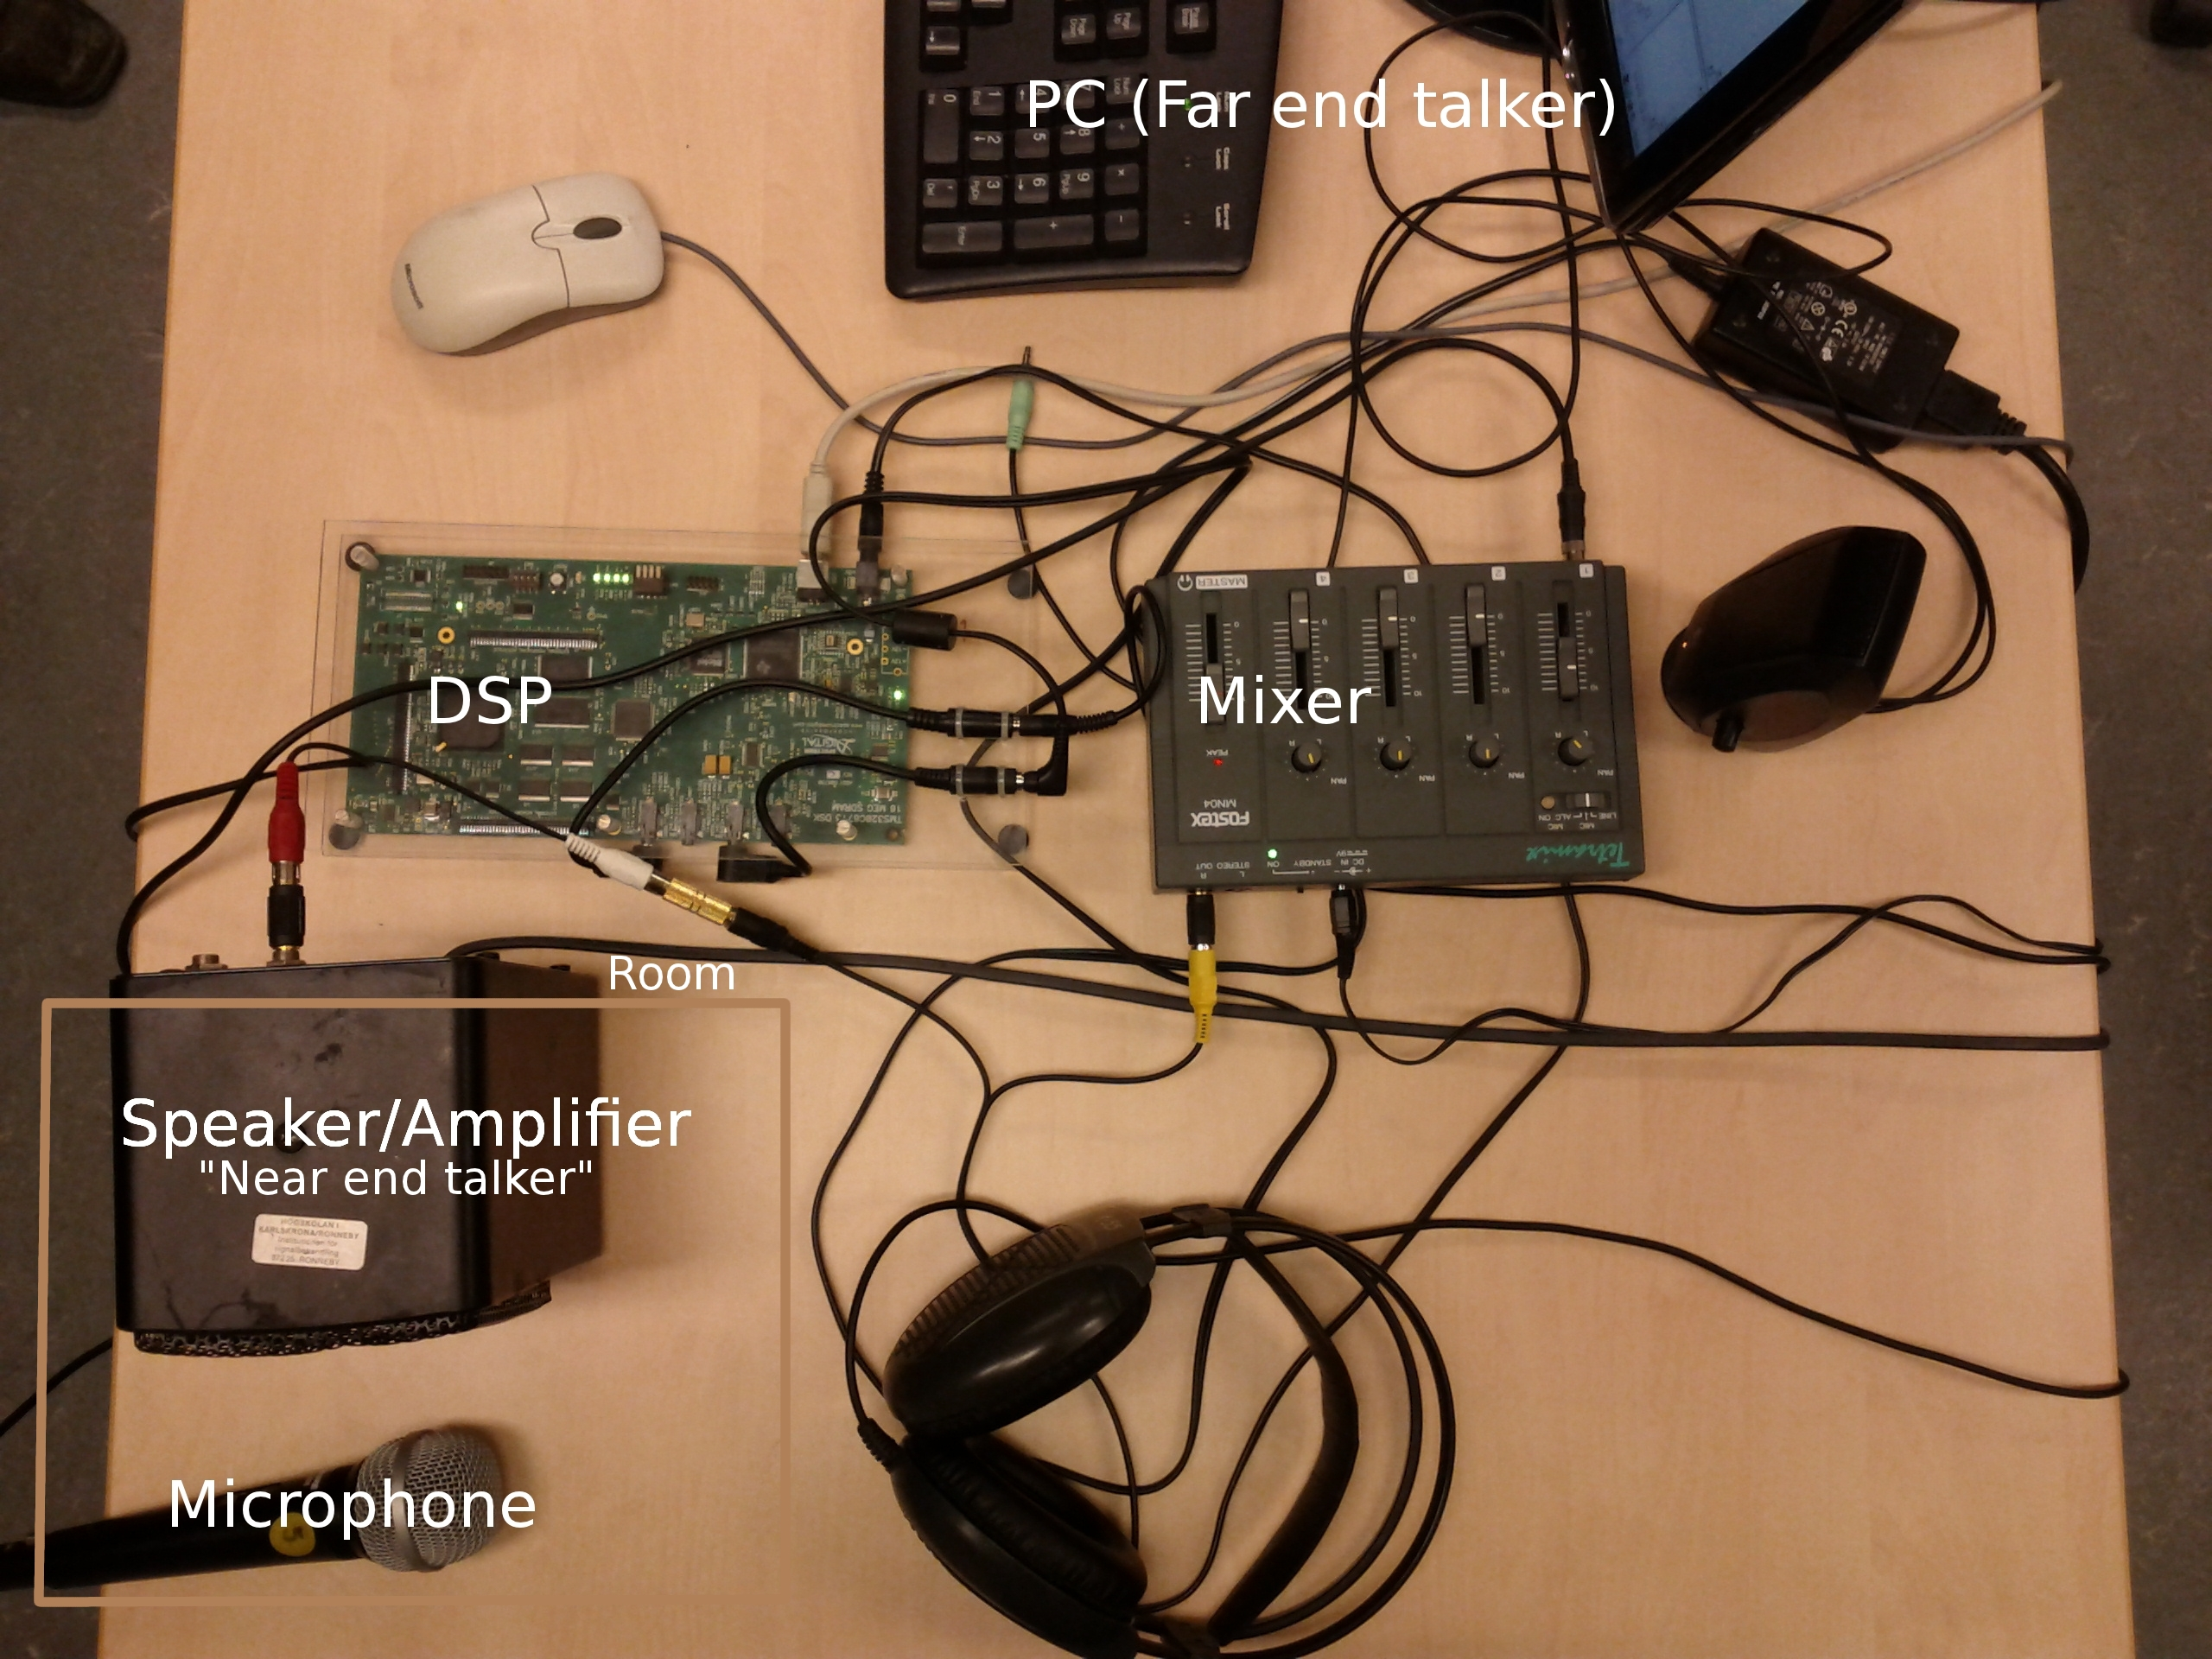
\includegraphics[width=1\textwidth]{apparatus.jpg}
  	\caption{An overview of the general setup environment for the Echo Cancellation project.}
\ \end{figure}

\section{Theory}
\label{sec:theory}

The sound from a speaker, for instance in a teleconferencing system,  gets reflected by the obstacles in a room like walls or other material surfaces. These reflected waves in turn get reflected and so on. This phenomenon creates an undesirable signal called echo which gets picked up by the microphone along with the desired signal of the near-end speaker. As such the sound quality received by the far-end listener gets reduced. The following subsection discusses a system implementing an adaptive filter algorithm to tackle the problem of removing the echo.

\subsection{Algorithm}

A high level block diagram of a system employing echo canceller is shown in figure \ref{fig:adaptive}. When the signal from the speaker passes through an air medium it does not follow a straight path, but rather gets reflected from different obstacles resulting in delayed versions of the signal. This delayed signal is what is called the echo as it will be picked by the microphone along with the near-end speaker which is the desired signal. Thus, the output of the system is the summation of the near-end signal and the echo. In order to extract only the near-end signal an adaptive filter that attempts to mimics the channel  is used. This filter adapts the behaviour of the system gradually by learning from the actual output. The filter mimics the echo of the system and outputs it, which is subtracted from the system output resulting in a signal close to the desired signal.

Adaptive filters is useful when the behaviour of the channel varies over time. Figure (M1) shows an adaptive echo cancellation system. In fact, the adaptive filter should remove the echoes comes from the speaker into the microphone. As shown in the figure, in the presence of the far-end signal, $x(t)$, the echo signal comes into the microphone which is filtered by the channel, $h_t$, which is modelled as n-tap FIR filter:

\begin{equation}\label{eq:n-tapFIR}
h = [ h(0) \ h(1)\dots \ h(n-1)] ^T   
\end{equation}

Then is the absence of near-end signal, $v(t)$, the output of the microphone is:

\begin{equation}
\ y(t) = h^T X(t) + w(t)\ 	
\end{equation}

Where $w(t)$ is the additive noise and:

 \begin{equation}
X(t) = [ x(t) \ x(t-1) \dots \ x(t-n+1) ]^T  
\end{equation}

If the adaptive filter tries to estimate the channel, $hat{h}$, as close as $h$, so the error will be the subtraction of microphone signal and the output of adaptive filter signal\cite{1}:

\begin{equation}
e(t) = y(t) - {\hat{h}}^{T} X(t)
\end{equation}

Some popular algorithms for the echo cancellation adaptive filters are LMS (NLMS) and RLS. The RLS method, is the most effective and robust but its more computational heavy which makes it unsuitable for use in an embedded system\cite{2}. Frequency-domain LMS algorithm is another sophisticated method for echo cancellation, because the time-domain impulse response of the speech (a non-stationary signal) requires very large filter taps. Also, the double talk separation in frequency domain\cite{3} is more easy than time-domain. A recently developed popular algorithm is the affine project algorithm (APA). The main advantage of this algorithm in comparison to NLMS is faster convergence rate, especially for speech signals\cite{4}.

\begin{figure} \
  \centering
	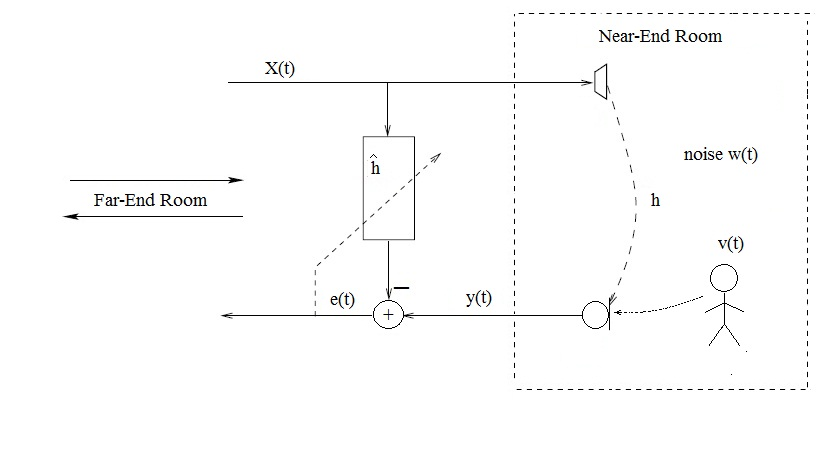
\includegraphics[width=1\textwidth]{Adaptive_Filter.jpg}
  	\caption{Adaptive filter\cite{1}.}
  	\label{fig:adaptive}
\ \end{figure}


\subsubsection{LMS}

% TODO: Write about the this algorithm/adaptive filter explaining with equations <Mahmoud?>

The least-mean-square (LMS) algorithm is one of the most popular adaptation algorithm for echo cancellation which have been used since in the mid 1960s\cite{5}. In adaptive filters the filter coefficients are updated as follow:

\begin{equation}
\hat{h}(n+1) = \hat{h}(n) + \Delta \hat{h} 
\end{equation}

 The LMS algorithm updates the filter coefficients  according to the negated gradient of mean square error as follows:

\begin{equation}
\Delta \hat{h} = - \frac{\mu}{2} \nabla E[e^2(n)] 
\end{equation}

where $\mu$ is the step size that indicate the rate of convergence, $\nabla$ is gradient and $E$ is the expectation of square error, but for LMS algorithm, the instantaneous value is replaced and after some manipulation the updated filter coefficients are:

\begin{equation}
\hat{h}(n+1) = \hat{h}(n) + \mu e(n) x(n) 
\end{equation}

\subsubsection{NLMS}
% TODO: Write about the this algorithm/adaptive filter explaining with equations, talking on limitation of LMS and then normalising with the input power <Mahmoud?>
There are some drawbacks in the LMS algorithm e.g that $\mu$ depends on the input vector; it means that for different values of the input signal, the step size should be changed, another one is that  the error is proportional to the input signal $x(n)$, then the updated part of the filter coefficients are proportional to the power of the input signal $x(n)$, and it suffers from the presence of noise. One way to avoid this problem in the normalized LMS is to normalize the updated part with the power of the input signal $x(n)$:

\begin{equation}
\hat{h}(n+1) = \hat{h}(n) + \frac{\mu}{\parallel x(n) \parallel ^2 + a}
\end{equation}

Where a is a protection value to avoid division by zero, in this approach $\mu$ can be between $0 < \mu < 2$.

 
% TODO: doubletalk - Do we need to talk about this? Are we doing anything about double talk in the final implementation?



% TODO: A block diagram of the final system and a few lines on the setup should be good.



\section{Simulation}
In the initial stage of the project it was essential to implement the algorithm in Matlab. Such an implementation would make it possible to compare the precision of the C implemented algorithm and plotting results in Matlab, which allows for more convenient error detection. By plotting the delta function it was possible to note the time instance of an echo's detection. The appearance of a new echo can be noticed through observation of the function's deviation at that point. Once the Matlab and C implementation to some extent match in term of efficiency and error parameters then the algorithm is deemed as stable and ready for implementation on the DSP board.

\subsection{Matlab}
%Choose an algorithm - NLMS
%implemented it in matlab
%tested it
%proceeded c implementation
%iteratively compared with matlab implementation

% TODO: A block diagram of the final system and a few lines on the setup should be good.
In order to generate the echoes the signal has to pass through the microphone 

As shown in figure \ref{fig:adaptive} the signal $X(t)$ travels through the channel which consequently picks up the noise $w(t)$ of the channel before it ends up at the microphone. Noside may come from the microphone, the environment and is dependent on the acoustics of the room. The inferred error is illustrated by figure \ref{fig:echoes} where the noise can be seen in the parts where there should be silence.

\begin{figure} \
  \centering

	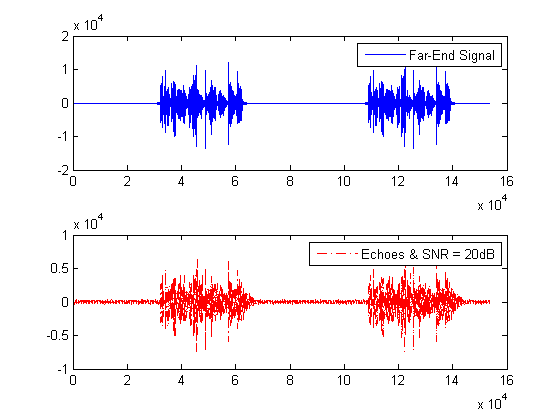
\includegraphics[width=1\textwidth]{Echoes.png}
  	\caption{Graph comparing the illustrated error before the speaker, and after the microphone.}
  	  \label{fig:echoes}
\ \end{figure}

Because of this noise the filter coefficients $\hat{h}$ will have a difficulty converging, so that the echo can be filtered correctly. The longer a signal has been received by the board the less it will be affected by the additive noise, because the taps will come closer to accurately approximating the channel. The error goes down as shown in figure \ref{fig:errors}.

\begin{figure} \label{fig:errors}\
  \centering
 
	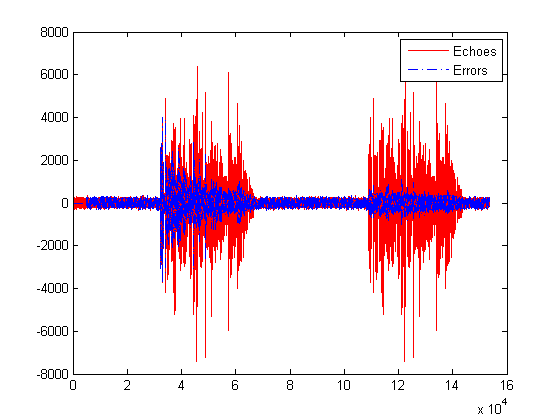
\includegraphics[width=1\textwidth]{Errors.png}
  	\caption{Shows graph of  coefficients $\hat{h}$ converging towards the channel over time.}
\ \end{figure}


\section{Implementation}
% difficulties, challanges, dev env, move to v5 of dev env, memory constraints,
% simulations, matlab, sampling frequency vs memory constraint, coversion to C,
% optimisation
% discuss the different optimisation techniques
\subsection{Hardware constraints}
The implementation of the algorithm was memory constraint-oriented. Due to the fact that the external DRAM memory proved to not be fast enough keeping all variables allocated on the stack was crucial. In order to keep such memory usage in check and be able to detect any spikes in such usage Code Composer Studio's CPU graph utility. Any CPU usage is displayed on the graph with CPU utilization on per-thread basis.

Greatest memory management improvement was observed once sampling frequency was lowered, which effectively lowered memory utilization, and allowed for a greater filter length. The latter provided a better performing echo canceller.

By using this information it was possible to push the size of the algorithm's adaptive coefficient vector to the out most limit without causing unnecessary crashes due to memory overflows.

\subsection{Optimizations in C}
By implementing the algorithm in C according to the sliding window principle it was possible to bring down the memory usage significantly. The algorithm is written such that the input signals are read once at most, upon which their results are computed and adaptive coefficients updated with each iteration.

\subsubsection{Signal threshold}
%threshold
%calculate the total variance(updated) variance of the block(current)
% when there's only noise - !update w[]
%far end talker - update
% doubletalk - do not update (not handled)
In order to cope with noise in the signal a signal threshold was introduced, which ideally would not allow background noise to pass through. if the near-end signal is and there for only noise is received then \texttt{w[]} coefficient vector, which is named $\hat{h}$ in section \ref{sec:theory} and equation \ref{eq:n-tapFIR}, should not be updated.

\begin{figure} \
  \centering  
	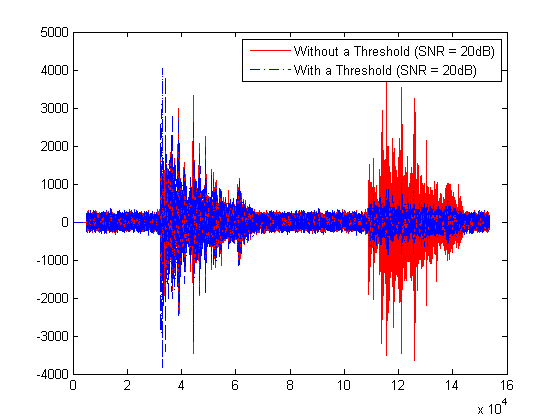
\includegraphics[width=1\textwidth]{Threshold.png}
  	\caption{Graph comparing error $e(t)$ signal threshold filter enabled, as opposed to disabled.}
  	\label{fig:threshold}
\ \end{figure}

According to figure \ref{fig:threshold} the error is unreasonably big if there is no threshold filter applied at the signal input block. Because the filter coefficients are updated when there is only noise present on the channel the coefficients are updated with the wrong audio data. This phenomenon is illustrated in figure \ref{fig:threshold} where the algorithm without the threshold filter presents significantly higher error values.

Therefore this graph shows that there is a need for a threshold which increases the overall accuracy of the echo canceller, which can also be seen in the figure. 

Once the far-end signal is larger then the noise threshold, the filter coefficients $\hat{h}$ should be updated again. However, the threshold is not a fixed variable but calculated according to a signal variance algorithm:

\begin{equation}
Th =  \frac{1}{N} \sum_{n=1}^{N} x(n)^2
\end{equation}

By using this algorithm the variance can be calculated for each audio block as well as the total number of audio blocks. Consequently the variance for total audio blocks and currently processed audio block will be compared according to:

\begin{equation}
Th_{total} > \frac{1}{N} \sum_{block = 1}^{block_{N}} x(n)^2
\end{equation}

Should the total variance of the audio blocks be bigger than the variance for the current block, then signal is deemed as noise.

\subsection{Problems}
During the development of the system several problems where encountered. To start off  the algorithm was implemented in a system agnostic way so as to allow regression testing against the Matlab implementation. This turned out to have been a very good choice as it was discovered that when something broke in the algorithm it was very seldom readily apparent. One example of such a devious error that occurred several times during different stages of the development of this project was that we accidentally introduced off by one errors when accessing the arrays. As we technically owned the memory accessed when running on the computer and the board lacks memory protection the program didn’t give us a segmentation fault or any other indication that something was amiss. The way we noticed these errors was that when the output of the C implementation was compared to the Matlab version we had minute errors in the output, had we simply ran it on the board everything would have appeared to be working except that the board could potentially have crashed at random intervals, in reality it did  not crash which means that such an error could easily have slip through to production code had we not had regression testing. Another difficulty that was encountered was that when something broke in the code it resulted in what appeared as random output meaning there was no easy way to tell what was wrong. We countered this by only changing small portions of the code at a time and continuous tests of the changes we made.


\section{Conclusion}
The goal of the project, to implement a working echo cancellation algorithm, was achieved as illustrated by figure \ref{fig:impulse}. It would have been good for the performance of the algorithm to implement double-talk\cite{1} detection. However,  the NLMS algorithm handles double-talk with sufficient accuracy for this project even without double talk detection. 

\begin{figure} \
  \centering  
	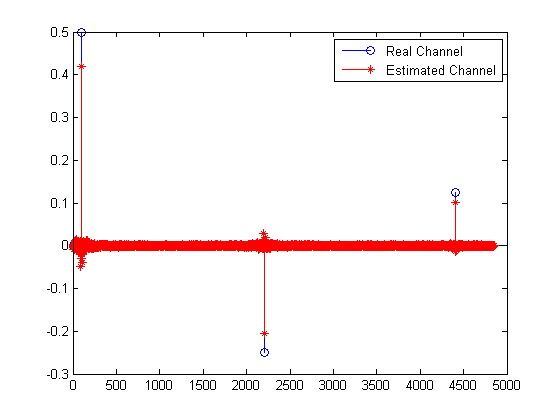
\includegraphics[width=1\textwidth]{Impuse_Response.png}
  	\caption{Channel estimation graph of C implementation (Estimated) compared to the real channel.}
  	\label{fig:impulse}
\ \end{figure}

%variable step size
%more mem filter length
% double talk
Due to the hardware constraints mentioned previously in the report, the filter length could not be larger than an array of 700 floating point integers. Because of this the amount of echoes that can be potentially detected may not exceed $87.5 \mu s$, which makes this another measure for the efficiency of the final filter.

Another improvement of this filter could have been made if a variable step-size algorithm was implemented, as it governs the rate of convergence towards the channel. This was not implemented due to the time constraint imposed by the project deadline.




%Make different parts of the document.
%Explain the theory, methods,
%implemetation, any databases, results, discussion, etc.
%
%Figures can be included, as in Figures~\ref{fig:smiley1} and~\ref{fig:smiley2}.
%
%Equations?
%\begin{equation}
%X(k) = \sum_{n=0}^{N-1} x[n] e^{-j2\pi nk/N}
%\end{equation}
%To cite recerences~\cite{Lindell99}, include them in the end:

\begin{thebibliography}{99}

\bibitem{1}
P. \o{A}hgren and A. Jakobsson,
\emph{A Study of Doubletalk Detection Performance in the Presence of Acoustic Path Changes},
IEEE Transaction on Consumer Electronics,
May 2006

\bibitem{2}
P. Sinha,
\emph{Speech Processing in Embedded System},
Springer, 
2010

\bibitem{3}
F. Capman, J. Boudy, P.Lockwood,
\emph{Acoustic Echo Cancellation and Noise Reduction in the Frequency-Domain: A Global Optimisation},

\bibitem{4}
C. Paleologu, J. Benesty, and S. Ciochina, 
\emph{Variable step-size affine projection algorithm designed for acoustic echo cancellation},
IEEE Trans. Audio, Speech, Language Process., 
Nov. 2008

\bibitem{5}
M. M. Sondhi, 
\emph{The History of Echo Cancellation},
IEEE Signal Processing Magazine,
Sept. 2006
\end{thebibliography}

\newpage
\section{Appendix - A}
\verbatiminput{code.c}
\end{document}
